\documentclass[Serif, 10pt, brown]{beamer}
\usepackage{booktabs,xcolor}
\usepackage{pifont}
\newcommand*\CHECK{\ding{51}}
\usepackage{array}
\newcolumntype{P}[1]{>{\centering\arraybackslash}p{#1}}
%
\usepackage{setspace,mathtools,amssymb,multirow,array,amsmath,tikz}
\usepackage[normalsize]{subfigure}
\usetikzlibrary{patterns}
\usetikzlibrary{automata,positioning,decorations.pathreplacing,decorations}

\usepackage{curves}
\usepackage{caption}
\usepackage{wasysym}
\usepackage{epsfig,epstopdf,graphicx}

\curvewarnfalse
%
\newtheorem{proposition}{Proposition}
\theoremstyle{example}
\newtheorem{theoremh}{Theorem}
\theoremstyle{plain}
\renewcommand{\textfraction}{0.01}
\renewcommand{\floatpagefraction}{0.99}
\newcommand{\ul}{\underline}
\newcounter{units}
\setbeamercovered{dynamic}
\logo{
\includegraphics[width=0.5in,keepaspectratio]{iitb_logo.png}}

\mode<presentation>
	{
\usetheme[right,currentsection, hideothersubsections]{UTD}
			\useoutertheme{sidebar} \useinnertheme[shadow]{rounded}
			\usecolortheme{whale} \usecolortheme{orchid}
			\usefonttheme[onlymath]{serif}
			\setbeamertemplate{footline}{\centerline{Slide \insertframenumber/\inserttotalframenumber}}
	}

\usebeamercolor[fg]{author in sidebar}
\title[{Systems for LLMs}]{\sc Benchmarking and Performance Analysis of LLM Inferencing Systems}
\author[\ul{Authors}]{{\textbf{Saksham Rathi}}}
\institute[UTD]{\sc\small Systems for LLMs\\ Under Prof. Mythili Vutukuru}
\date[UCI]{Indian Institute of Technology Bombay \\ Autumn 2025-26}

\begin{document}
\frame{\titlepage}

\begin{frame}{Contents}
	\tableofcontents
\end{frame}

\section{Workload Picked}
\begin{frame}{Workload Picked}
    \begin{itemize}
        \item Targeted a very specific workload
        \item Large system prompt ($\approx$ 1500 tokens) containing useful context and shared across all the queries
        \item Varying query input rate (from 5 req/sec to 700 req/sec)
        \item Small query sizes (10 to 20 tokens each) and small output requirements (capped at 30 to 50 tokens)
        \item Ideally, prefix sharing should help a lot
        \item \textbf{Next Step:} Family of requests, each family with a particular large system prompt and a few queries
    \end{itemize}
\end{frame}

\section{Batch of requests through various Engines}
\begin{frame}{Batch of requests through various Engines}

\begin{table}[h]
\centering
\begin{tabular}{|l|c|}
\hline
\textbf{Technique Used} & \textbf{Time (s)} \\
\hline
Transformers (batch size = 1) & 30.21 \\
Transformers (batch size = 2) & 19.51 \\
Transformers (batch size = 3) & 18.64 \\
vLLM (no system prompt pre-filling) & 0.45 \\
SGLang (fork) & 1.03 \\
SGLang (run\_batch) & 0.40 \\
NEO & 0.55 \\
\hline
\end{tabular}
\caption{Measuring the time taken to process a batch of 24 requests using different techniques}
\end{table}
    
\end{frame}

\begin{frame}{Batch of requests through various Engines}
    \begin{columns}[T, totalwidth=\textwidth]
        \begin{column}{0.6\textwidth}
            \centering
            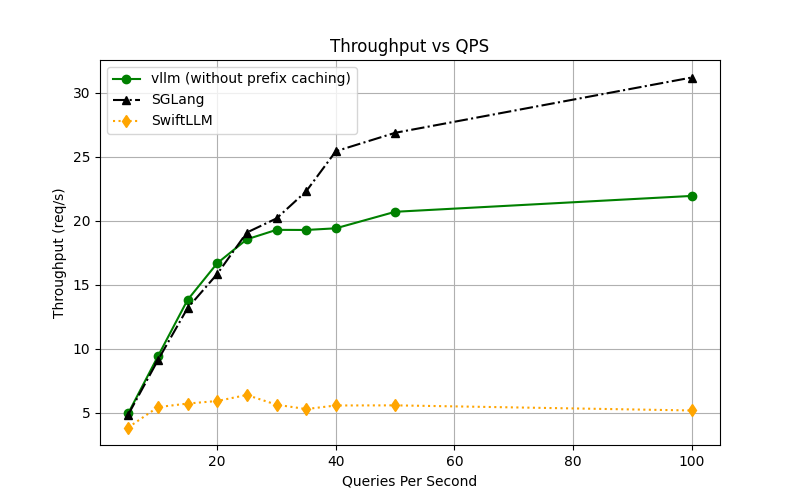
\includegraphics[width=\textwidth]{../results/throughput_vs_qps.png}
            \vspace{0.3em}
            \captionof{figure}{Throughput comparison across varying workloads}
        \end{column}
        \begin{column}{0.4\textwidth}
            \begin{itemize}
                \item SwiftLLM is a small copy (2000 lines of code) of vLLM, promises to perform equivalent to vLLM.
                \item SGLANG performs quite better because of prefix sharing through radix tree.
            \end{itemize}
        \end{column}
    \end{columns}
\end{frame}

\begin{frame}{Batch of requests through various Engines}
    \begin{figure}[h]
    \centering
    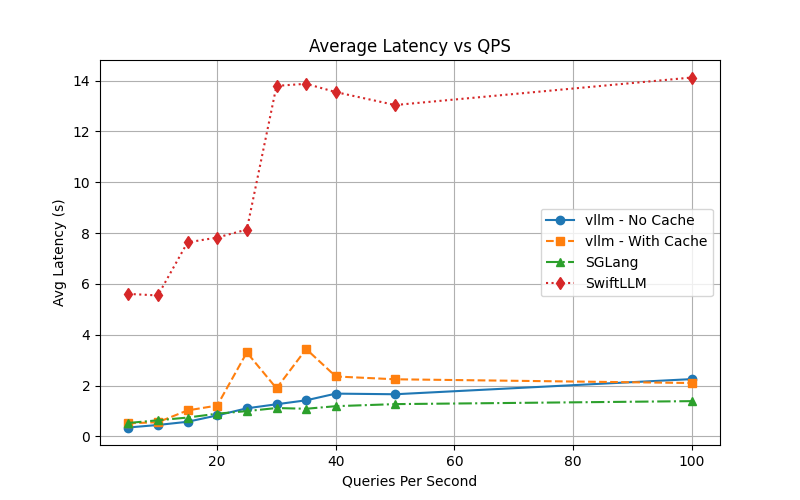
\includegraphics[width=0.7\textwidth]{../results/avg_latency_vs_qps.png}
    \caption{Average Latency comparison across varying workloads}
\end{figure}
\end{frame}

\section{LLM Request Timelines}
\begin{frame}{LLM Request Timelines}
    \begin{columns}[T, totalwidth=\textwidth]
        \begin{column}{0.6\textwidth}
            \centering
            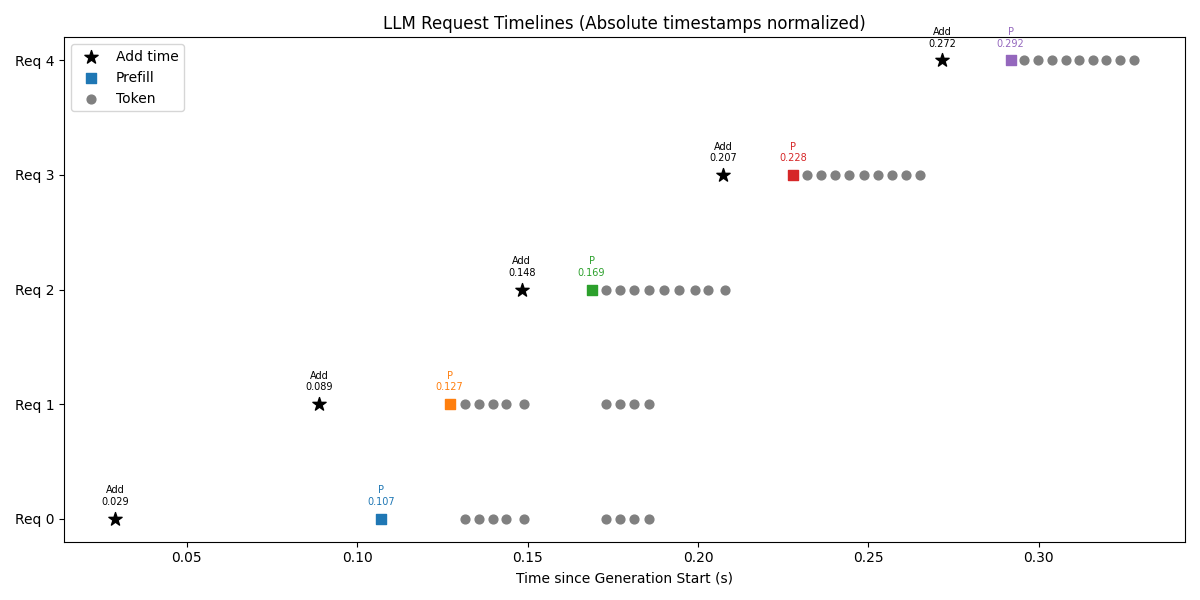
\includegraphics[width=\textwidth]{figures/llm_timelines_20.png}
            \vspace{0.3em}
            \captionof{figure}{20 Requests per second — without chunked prefill — vLLM V0 Engine}
        \end{column}
        \begin{column}{0.4\textwidth}
            \begin{itemize}
                \item Prefills take too much time as compared to decodes, primiarily because of large system prompt size.
                \item In this mode prefills can't go along with decodes.
                \item Prefills are preferred over decodes to reduce TTFT but total response time is quite high.
            \end{itemize}
        \end{column}
    \end{columns}
\end{frame}


\section{NSYS Measurements}
\begin{frame}{NSYS Measurements}
    \begin{figure}[h]
    \centering
    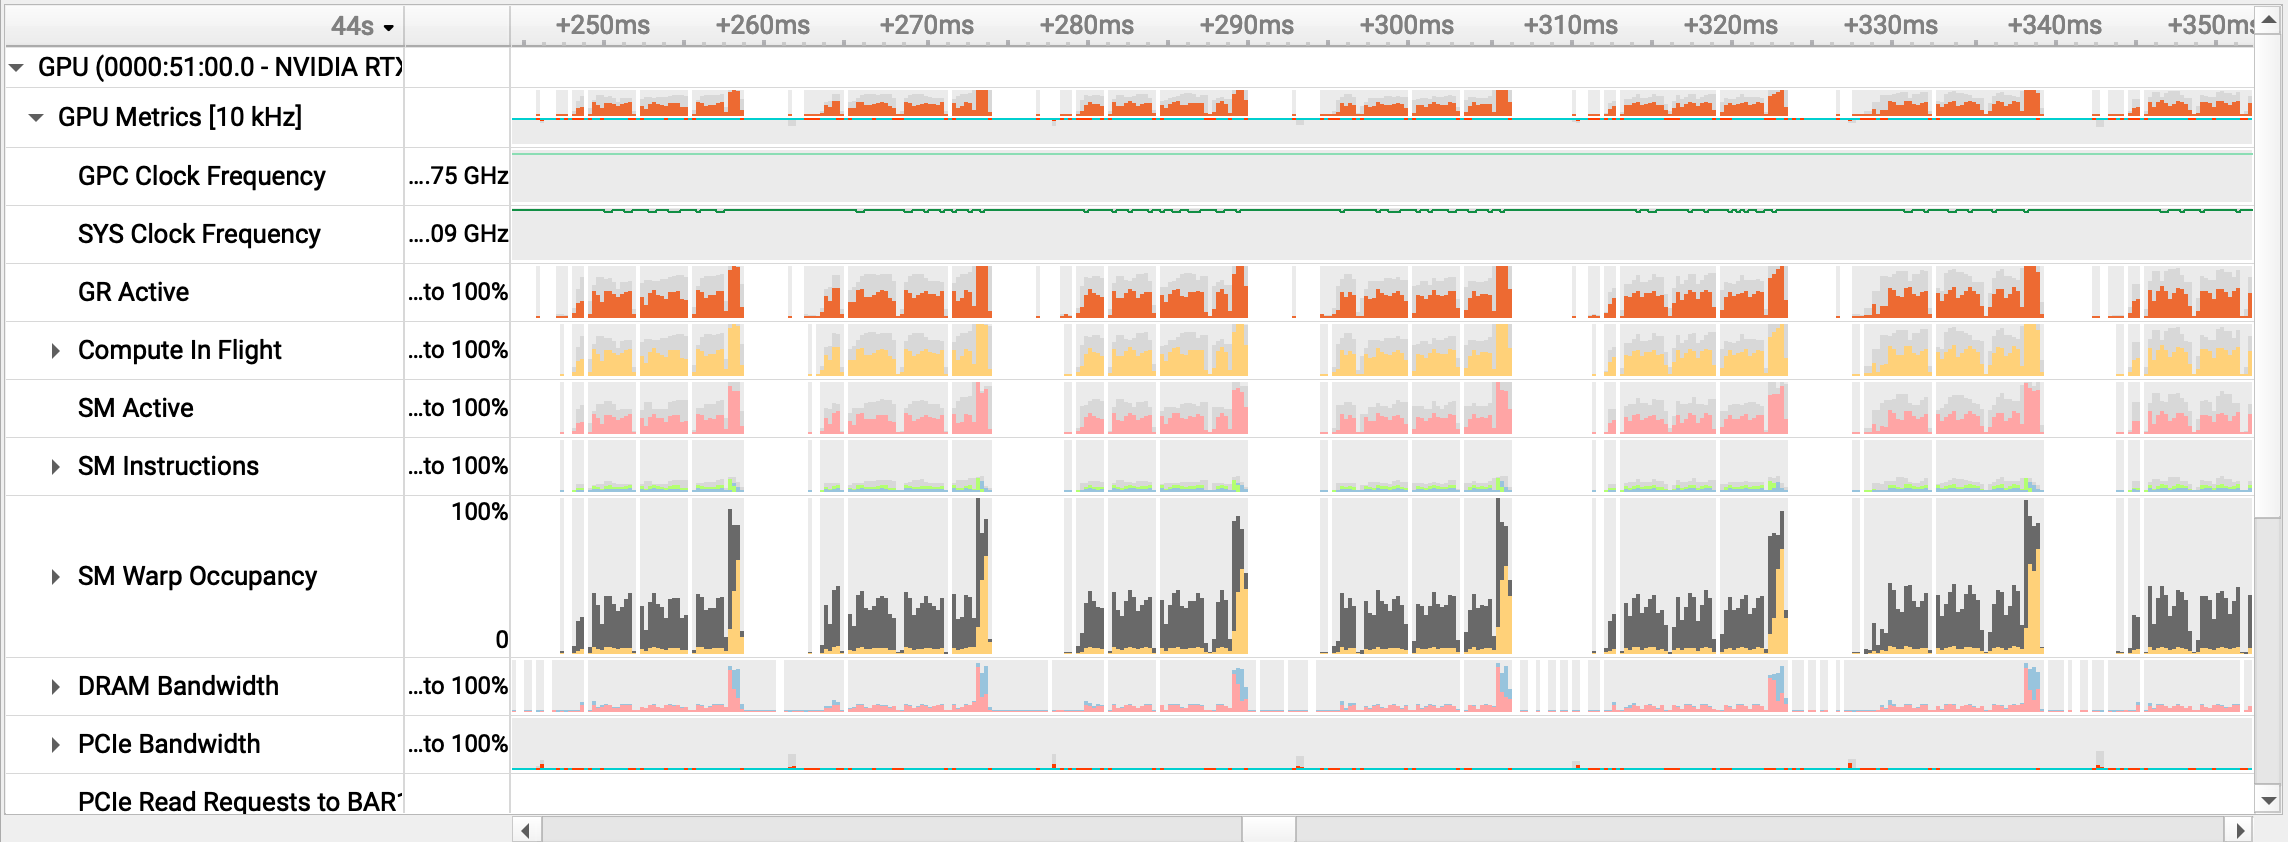
\includegraphics[width=0.7\textwidth]{../results/nsys_metrics_llm_inference.png}
    \caption{NSYS Metrics Snapshot}
\end{figure}

\begin{itemize}
    \item For compute: we just check SM Active and Warp occupancy.
    \item For memory: vLLM books all the available memory in the start, scheduler stats show the actual KV Cache usage.
    \item PCIe Bandwidth isn't utilized fully - small workloads - no need to transfer stuff to CPU.
\end{itemize}
\end{frame}

\section{Throughput vs Load for vLLM}

\begin{frame}{Throughput vs Load for vLLM}
    \begin{columns}[T, totalwidth=\textwidth]
        \begin{column}{0.6\textwidth}
            \centering
            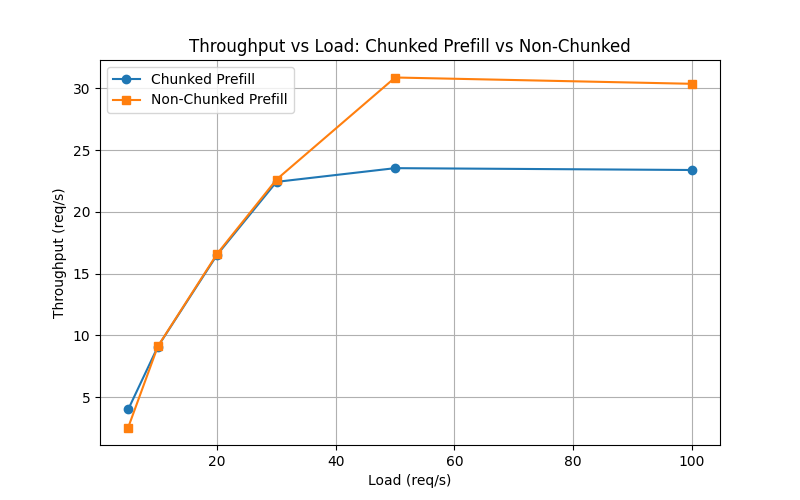
\includegraphics[width=\textwidth]{../results/throughput_comparison_vllm.png}
            \captionof{figure}{Throughput vs Load}
        \end{column}
        \begin{column}{0.4\textwidth}
            \begin{itemize}
                \item Chunked prefill does not really help that much for our type of workload.
                \item Prefix caching helps a lot, as is visible from the immense difference in throughputs.
                \item By changing the batch size (in terms of number of sequences and the token budget), we can achieve higher throughputs too.
            \end{itemize}
        \end{column}
    \end{columns}
\end{frame}

\section{GPU Memory Breakdown}

\begin{frame}{GPU Memory Breakdown}
    \begin{table}[h!]
\centering
\begin{tabular}{|c|p{4cm}|}
\hline
\textbf{Component} & \textbf{Memory Occupied} \\
\hline
Weights  & 0.93 GiB \\
\hline
Peak Activation  & 4.07 GiB \\
\hline
Non-Torch  & 0.02 GiB \\
\hline
CUDA Graph & 0.41 GiB \\
\hline
KV Cache: Intersection (Prefix)  & 1,280 tokens / 0.0157 GiB \\
\hline
KV Cache: Extras for Requests  & 640 tokens (10 requests × 64 tokens) / 0.0078 GiB \\
\hline
KV Cache: Free & 2,672,880 tokens / 32.8445 GiB \\
\hline
\end{tabular}
\caption{GPU Memory Breakdown and KV Cache Usage}
\label{tab:gpu_memory_breakdown}
\end{table}
\end{frame}


\section{Future Steps}
\begin{frame}{Future Steps}
\begin{itemize}
    \item Find the max throughput we can achieve for this kind of workload through vLLM
    \item Find the throughput for a family of requests, each family sharing a system prompt amongst its members
    \item Explore other batching techniques for such a family of requests, taking prefix sharing into consideration
    \item Possible changes to the scheduling algorithm
    \item Can we offload stuff to CPU, when we have computed the KV Cache, and we just need to perform decode operations?
    \item Possible optimizations to fine tuning
\end{itemize}
\end{frame}

\section{}
\begin{frame}
    \Huge{\centerline{\bf Thank You}}
\end{frame}

\end{document}


